%%%%%%%%%%%%%%%%%%%%%%%%%%%%%%%%%%%%%%%%%
% Short Sectioned Assignment
% LaTeX Template
% Version 1.0 (5/5/12)
%
% This template has been downloaded from:
% http://www.LaTeXTemplates.com
%
% Original author:
% Frits Wenneker (http://www.howtotex.com)
%
% License:
% CC BY-NC-SA 3.0 (http://creativecommons.org/licenses/by-nc-sa/3.0/)
%
%%%%%%%%%%%%%%%%%%%%%%%%%%%%%%%%%%%%%%%%%

%----------------------------------------------------------------------------------------
%	PACKAGES AND OTHER DOCUMENT CONFIGURATIONS
%----------------------------------------------------------------------------------------

\documentclass[paper=a4, fontsize=11pt]{scrartcl} % A4 paper and 11pt font size

\usepackage[T1]{fontenc} % Use 8-bit encoding that has 256 glyphs
%\usepackage{fourier} % Use the Adobe Utopia font for the document - comment this line to return to the LaTeX default
\usepackage[english]{babel} % English language/hyphenation
\usepackage[utf8]{inputenc}  %allows non-English characters
\usepackage{amsmath,amsfonts,amsthm} % Math packages

\usepackage{sectsty} % Allows customizing section commands
%\allsectionsfont{\centering \normalfont\scshape} % Make all sections centered, the default font and small caps
\allsectionsfont{\centering}

\usepackage{fancyhdr} % Custom headers and footers
\pagestyle{fancyplain} % Makes all pages in the document conform to the custom headers and footers
\fancyhead{} % No page header - if you want one, create it in the same way as the footers below
\fancyfoot[L]{} % Empty left footer
\fancyfoot[C]{} % Empty center footer
\fancyfoot[R]{\thepage} % Page numbering for right footer
\renewcommand{\headrulewidth}{0pt} % Remove header underlines
\renewcommand{\footrulewidth}{0pt} % Remove footer underlines
\setlength{\headheight}{13.6pt} % Customize the height of the header

%\usepackage{geometry}
%\usepackage{pdflscape}


%\numberwithin{equation}{section} % Number equations within sections (i.e. 1.1, 1.2, 2.1, 2.2 instead of 1, 2, 3, 4)
%\numberwithin{figure}{section} % Number figures within sections (i.e. 1.1, 1.2, 2.1, 2.2 instead of 1, 2, 3, 4)
%\numberwithin{table}{section} % Number tables within sections (i.e. 1.1, 1.2, 2.1, 2.2 instead of 1, 2, 3, 4)

%\setlength\parindent{0pt} % Removes all indentation from paragraphs - comment this line for an assignment with lots of text

\usepackage{caption}
%\usepackage{topcapt}

\usepackage{booktabs}

\usepackage{graphicx}
\usepackage{adjustbox}
\graphicspath{{../data/}}


%shortcuts for typing variance and expectation
\newcommand{\E}{\mathrm{E}}
\newcommand{\Var}{\mathrm{Var}}

%----------------------------------------------------------------------------------------
%	TITLE SECTION
%----------------------------------------------------------------------------------------

\newcommand{\horrule}[1]{\rule{\linewidth}{#1}} % Create horizontal rule command with 1 argument of height

\title{
\normalfont \normalsize
\textsc{UPC - Complex and Social Networks} \\ [25pt] % Your university, school and/or department name(s)
\horrule{0.5pt} \\[0.4cm] % Thin top horizontal rule
\huge Lab5: Finding community structures \\ % The assignment title
\horrule{2pt} \\[0.5cm] % Thick bottom horizontal rule
}

\author{Jakub Šalagovič\\Simon Van den Eynde} % Your name

\date{\normalsize\today} % Today's date or a custom date

\begin{document}


\maketitle % Print the title


%----------------------------------------------------------------------------------------
%	INTRO
%----------------------------------------------------------------------------------------

\section{Introduction}
This report exists of $2$ parts. In the first part we will compare some of igraph's community-finding algorithms on specifically chosen graphs, using the metrics: Triangle Partition Ratio (high is best), expansion (low is best), conductance (low is best) and modularity (high is best).
\section{Results}
% latex table generated in R 3.1.2 by xtable 1.8-2 package
% Wed Nov 23 21:28:34 2016
\begin{table}[ht]
\centering
\begin{tabular}{rrrrr}
  \hline
 & TPT & expansion & conductance & modularity \\ 
  \hline
edge.betweenness & 1.000 & 4.400 & 0.524 & 0.425 \\ 
  
             fastgreedy & 1.000 & 4.400 & 0.524 & 0.425 \\ 
  
             label.propagation & 1.000 & 4.160 & 0.482 & 0.340 \\ 
  
             leading.eigenvector & 1.000 & 3.200 & 0.333 & 0.000 \\ 
  
             multilevel & 1.000 & 4.400 & 0.524 & 0.425 \\ 
  
             optimal & 1.000 & 4.400 & 0.524 & 0.425 \\ 
  
             spinglass & 1.000 & 4.400 & 0.524 & 0.425 \\ 
  
             walktrap & 1.000 & 4.400 & 0.524 & 0.425 \\ 
  
             infomap & 1.000 & 4.400 & 0.524 & 0.425 \\ 
   \hline
\end{tabular}
\caption{Metrics for HanoiTower(5,2) (HT)} 
\end{table}
% latex table generated in R 3.1.2 by xtable 1.8-2 package
% Wed Nov 23 21:28:34 2016
\begin{table}[ht]
\centering
\begin{tabular}{rrrrr}
  \hline
 & TPT & expansion & conductance & modularity \\ 
  \hline
edge.betweenness & 0.000 & 1.933 & 0.476 & 0.451 \\ 
  
             fastgreedy & 0.000 & 2.000 & 0.501 & 0.411 \\ 
  
             label.propagation & 0.000 & 1.800 & 0.430 & 0.420 \\ 
  
             leading.eigenvector & 0.000 & 1.667 & 0.385 & 0.389 \\ 
  
             multilevel & 0.000 & 1.933 & 0.476 & 0.451 \\ 
  
             optimal & 0.000 & 1.933 & 0.476 & 0.451 \\ 
  
             spinglass & 0.000 & 2.067 & 0.527 & 0.442 \\ 
  
             walktrap & 0.000 & 1.933 & 0.476 & 0.451 \\ 
  
             infomap & 0.000 & 1.867 & 0.456 & 0.416 \\ 
   \hline
\end{tabular}
\caption{Metrics for Double Star Snark (DSS)} 
\end{table}
% latex table generated in R 3.1.2 by xtable 1.8-2 package
% Wed Nov 23 21:28:34 2016
\begin{table}[ht]
\centering
\begin{tabular}{rrrrr}
  \hline
 & TPT & expansion & conductance & modularity \\ 
  \hline
edge.betweenness & 0.600 & 2.467 & 0.529 & 0.228 \\ 
  
             fastgreedy & 0.400 & 2.733 & 0.609 & 0.217 \\ 
  
             label.propagation & 1.000 & 1.800 & 0.333 & 0.000 \\ 
  
             leading.eigenvector & 1.000 & 1.800 & 0.333 & 0.000 \\ 
  
             multilevel & 0.600 & 2.600 & 0.565 & 0.222 \\ 
  
             optimal & 0.600 & 2.467 & 0.530 & 0.239 \\ 
  
             spinglass & 0.400 & 2.600 & 0.577 & 0.230 \\ 
  
             walktrap & 0.400 & 2.600 & 0.575 & 0.181 \\ 
  
             infomap & 1.000 & 1.800 & 0.333 & 0.000 \\ 
   \hline
\end{tabular}
\caption{Metrics for the Dorovtsev-Goltsev-Mendes(3) Graph (DGM)} 
\end{table}
% latex table generated in R 3.1.2 by xtable 1.8-2 package
% Wed Nov 23 21:28:35 2016
\begin{table}[ht]
\centering
\begin{tabular}{rrrrr}
  \hline
 & TPT & expansion & conductance & modularity \\ 
  \hline
edge.betweenness & 0.000 & 1.075 & 0.381 & 0.680 \\ 
  
             fastgreedy & 0.000 & 1.100 & 0.393 & 0.678 \\ 
  
             label.propagation & 0.000 & 1.200 & 0.451 & 0.614 \\ 
  
             leading.eigenvector & 0.000 & 1.075 & 0.381 & 0.680 \\ 
  
             multilevel & 0.000 & 1.100 & 0.393 & 0.678 \\ 
  
             optimal & 0.000 & 1.075 & 0.381 & 0.680 \\ 
  
             spinglass & 0.000 & 1.100 & 0.393 & 0.678 \\ 
  
             walktrap & 0.000 & 1.125 & 0.406 & 0.652 \\ 
  
             infomap & 0.000 & 1.125 & 0.406 & 0.670 \\ 
   \hline
\end{tabular}
\caption{Metrics for Barabasi-Albert (BA)} 
\end{table}
% latex table generated in R 3.1.2 by xtable 1.8-2 package
% Wed Nov 23 21:28:35 2016
\begin{table}[ht]
\centering
\begin{tabular}{rrrrr}
  \hline
 & TPT & expansion & conductance & modularity \\ 
  \hline
edge.betweenness & 0.794 & 3.000 & 0.497 & 0.401 \\ 
  
             fastgreedy & 0.824 & 2.853 & 0.454 & 0.381 \\ 
  
             label.propagation & 0.882 & 2.706 & 0.427 & 0.338 \\ 
  
             leading.eigenvector & 0.735 & 3.059 & 0.502 & 0.393 \\ 
  
             multilevel & 0.794 & 2.912 & 0.468 & 0.419 \\ 
  
             optimal & 0.794 & 2.912 & 0.468 & 0.420 \\ 
  
             spinglass & 0.794 & 2.912 & 0.468 & 0.420 \\ 
  
             walktrap & 0.588 & 3.235 & 0.545 & 0.353 \\ 
  
             infomap & 0.882 & 2.706 & 0.419 & 0.402 \\ 
   \hline
\end{tabular}
\caption{Metrics for Zachary's Karate network (ZK)} 
\end{table}

\newpage

\section{Discussion}
For more information on the chosen graphs, see section \ref{meth}. 
\begin{itemize}
\item In general we notice that the modularity sometimes becomes zero, this happens only if the entire network is one community. In this case we can discard these findings.
\item In graphs without triangles (BA, DSS) or with many triangles (HT) we find that that the Triangle Partition Ratio does not convey any useful information.
\item We see that for if there are clear communities as in HT, almost every community-finding method can identify them correctly.
\item When looking at the metric values for the DSS network, we see that the leading.eigenvalue gives rise a special community structure. Its expansion and conductance are a lot lower than for other graphs, which is good. But its modularity is also a lot lower, which is a bad sign. When comparing network sizes (not included) we note it is the only community structure which consists of only $2$ communities. So depending on how many communities you want, you might consider using different metrics our different community-finding methods.
\item The values for the conductance and expansion of the BA network are lower than that of other networks. Also the modularity is higher. This means that this power-law delivers stronger communities than many other graphs.
\end{itemize}


\section{Methods}\label{meth}
\subsection{Graphs}
We chose 5 different graphs. As a real network we chose Zachary's karate (ZK) network. We also analysed a Barab\'{a}si-Albert (BA) graph on $40$ vertices.
Furthermore we considered $3$ special graphs:
\paragraph{HanoiTower(5,2) (HT)}
This graph has as nodes the game states of Hanoi Tower game with $5$ pegs and $2$ disks, there is an edge if you can go from one game state to another in one move. This graph basically consists of $5$ copies of $K_{5}$ which are sparsely connected. See figure~\ref{ht}.
\paragraph{Double Star Snark (DSS)} This is graph is snark, which means it doesn't contain any triangle (this graph does only contain cycles with length $>5$), it is also cubic and has no bridges. It consists of $30$ vertices. See figure~\ref{dss}.
\paragraph{Dorovstev-Goltsev-Mendes graph (DGM)} This is a graph which can be constructed, starting with $K_{2}$, as follows: for every edge a triangle (add a vertex and 2 edges). If we do this $3$ times we get a graph with $15$ vertices, $27$ edges and a lot of triangles. See figure~\ref{dgm}.

%\paragraph{Randomization}
%For the standard graphs we chose (Hanoi Tower, double star snark and the Dorovstev-Goltsev-Mendes graph), we got counterintuitive results for our metrics. Because these graphs have many automorfisms and this is not so realistic, we randomised these networks. To do so, we rewired $15\%$ of all edges of these graphs.

\begin{figure}[htbp]
   \centering
   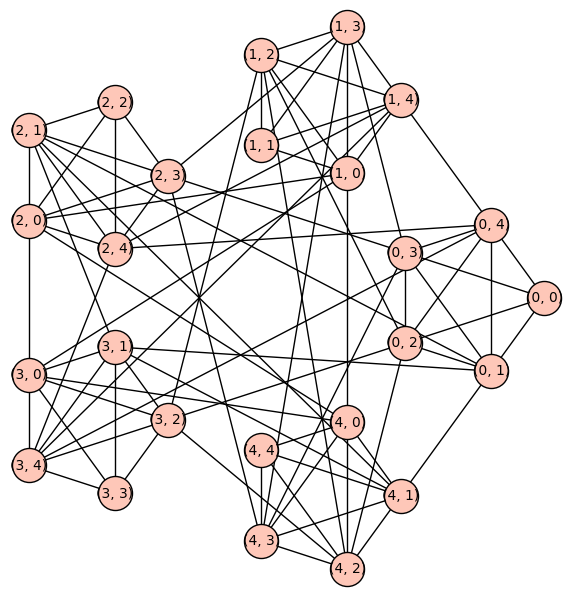
\includegraphics{ht} % requires the graphicx package
   \caption{The Hanoi Tower graph with $5$ pegs and $2$ discs. The labels on the vertices indicate the positions of the two discs ($(1,3)$ means: peg $1$ on disk $1$, peg $2$ on disc $2$)}
   \label{ht}
\end{figure}
\begin{figure}[htbp]
   \centering
   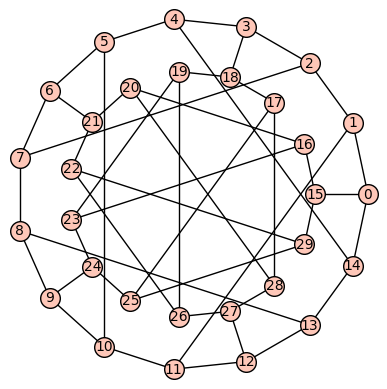
\includegraphics{dss} % requires the graphicx package
   \caption{The double star snark}
   \label{dss}
\end{figure}

\begin{figure}[htbp]
   \centering
   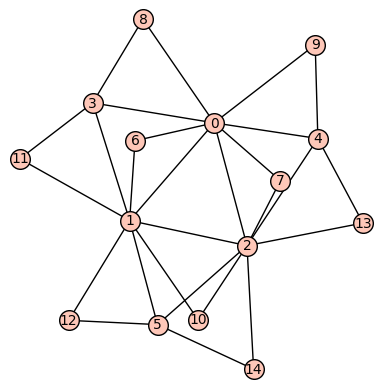
\includegraphics{dgm} % requires the graphicx package
   \caption{The Dorovstev-Goltsev-Mendes graph after $3$ iterations}
   \label{dgm}
\end{figure}


\section{Appendix}

\end{document}
